\documentclass{beamer} % descomentar para tener pausas
% \documentclass[handout]{beamer} % descomentar para no tener pausas
\usetheme{CambridgeUS}
\setbeamertemplate{background}[grid][step=8 ] % cuadriculado


\usepackage[utf8]{inputenc} %esto permite (en Windows) escribir directamente 
\usepackage{graphicx}
\usepackage{array}
\usepackage{tikz} 
\usetikzlibrary{shapes,arrows,babel,decorations.pathreplacing}
\usepackage{verbatim} 
\usepackage{xcolor} 
\usepackage{amsgen,amsmath,amstext,amsbsy,amsopn,amsfonts,amssymb}
\usepackage{amsthm}
\usepackage{tikz}
\usepackage{tkz-graph}
\usepackage{mathtools}
\usepackage{xcolor}

%\setbeamertemplate{background}[grid][step=8 ]
\setbeamertemplate{itemize item}{$\circ$}
\setbeamertemplate{enumerate items}[default]

\definecolor{links}{HTML}{2A1B81}
\hypersetup{colorlinks,linkcolor=,urlcolor=links}

\newcommand{\img}{\operatorname{Im}}
\newcommand{\nuc}{\operatorname{Nu}}
\newcommand\im{\operatorname{Im}}
\renewcommand\nu{\operatorname{Nu}}
\newcommand{\la}{\langle}
\newcommand{\ra}{\rangle}
\renewcommand{\t}{{\operatorname{t}}}
\renewcommand{\sin}{{\,\operatorname{sen}}}
\newcommand{\Q}{\mathbb Q}
\newcommand{\R}{\mathbb R}
\newcommand{\C}{\mathbb C}
\newcommand{\K}{\mathbb K}
\newcommand{\F}{\mathbb F}
\newcommand{\Z}{\mathbb Z}

\renewcommand{\figurename }{Figura}
%\usepackage{enumitem}
%\setlist[itemize]{itemsep=10pt, label={$\circ$}}
%\newtheorem{teorema}{Teorema}
%\newtheorem{corolario}[teorema]{Corolario}
%\newtheorem{proposicion}[teorema]{Proposición}

%\theoremstyle{definition}
%\newtheorem{definicion}[theorem]{Definición}
%\newtheorem{ejemplo}[theorem]{Ejemplo}
%\newtheorem{pregunta}[equation]{Pregunta}
%\newtheorem{step}{Paso}



\newenvironment{exercise}[1]% environment name
{% begin code
    \par\vspace{\baselineskip}\noindent
    \textbf{Ejercicio (#1)}\begin{itshape}%
        \par\vspace{\baselineskip}\noindent\ignorespaces
    }%
    {% end code
    \end{itshape}\ignorespacesafterend
}


\newenvironment{definicion}% environment name
{% begin code
    \par\vskip .2cm%
    {\color{blue}Definición}%
    \vskip .2cm
}%
{%
    \vskip .2cm}% end code

\newenvironment{observacion}% environment name
{% begin code
    \par\vskip .2cm%
    {\color{blue}Observación}%
    \vskip .2cm
}%
{%
    \vskip .2cm}% end code

\newenvironment{ejemplo}% environment name
{% begin code
    \par\vskip .2cm%
    {\color{blue}Ejemplo}%
    \vskip .2cm
}%
{%
    \vskip .2cm}% end code

\newenvironment{ejercicio}% environment name
{% begin code
    \par\vskip .2cm%
    {\color{blue}Ejercicio}%
    \vskip .2cm
}%
{%
    \vskip .2cm}% end code


\renewenvironment{proof}% environment name
{% begin code
    \par\vskip .2cm%
    {\color{blue}Demostración}%
    \vskip .2cm
}%
{%
    \vskip .2cm}% end code



\newenvironment{demostracion}% environment name
{% begin code
    \par\vskip .2cm%
    {\color{blue}Demostración}%
    \vskip .2cm
}%
{%
    \vskip .2cm}% end code

\newenvironment{idea}% environment name
{% begin code
    \par\vskip .2cm%
    {\color{blue}Idea de la demostración}%
    \vskip .2cm
}%
{%
    \vskip .2cm}% end code

\newenvironment{solucion}% environment name
{% begin code
    \par\vskip .2cm%
    {\color{blue}Solución}%
    \vskip .2cm
}%
{%
    \vskip .2cm}% end code



\newenvironment{lema}% environment name
{% begin code
    \par\vskip .2cm%
    {\color{blue}Lema}\begin{itshape}%
        \par\vskip .2cm
    }%
    {% end code
    \end{itshape}\vskip .2cm\ignorespacesafterend
}

\newenvironment{proposicion}% environment name
{% begin code
    \par\vskip .2cm%
    {\color{blue}Proposición}\begin{itshape}%
        \par\vskip .2cm
    }%
    {% end code
    \end{itshape}\vskip .2cm\ignorespacesafterend
}

\newenvironment{teorema}% environment name
{% begin code
    \par\vskip .2cm%
    {\color{blue}Teorema}\begin{itshape}%
        \par\vskip .2cm
    }%
    {% end code
    \end{itshape}\vskip .2cm\ignorespacesafterend
}


\newenvironment{corolario}% environment name
{% begin code
    \par\vskip .2cm%
    {\color{blue}Corolario}\begin{itshape}%
        \par\vskip .2cm
    }%
    {% end code
    \end{itshape}\vskip .2cm\ignorespacesafterend
}

\newenvironment{propiedad}% environment name
{% begin code
    \par\vskip .2cm%
    {\color{blue}Propiedad}\begin{itshape}%
        \par\vskip .2cm
    }%
    {% end code
    \end{itshape}\vskip .2cm\ignorespacesafterend
}


\setbeamercolor{block}{fg=red, bg=red!40!white}
\setbeamercolor{block example}{use=structure,fg=black,bg=white!20!white}

\renewenvironment{block}[1]% environment name
{% begin code
    \par\vskip .2cm%
    {\color{blue}#1}%
    \vskip .2cm
}%
{%
    \vskip .2cm}% end code


\renewenvironment{alertblock}[1]% environment name
{% begin code
    \par\vskip .2cm%
    {\color{red!80!black}#1}%
    \vskip .2cm
}%
{%
    \vskip .2cm}% end code


\renewenvironment{exampleblock}[1]% environment name
{% begin code
    \par\vskip .2cm%
    {\color{blue}#1}%
    \vskip .2cm
}%
{%
    \vskip .2cm}% end code
%%%%%%%%%%%%%%%%%%%%%%%%%%%%%%%%%%%%%%%%%%%%%%%%%%%%%%%


\title[Clase 1 - Vectores en $\R^2$ y $\R^3$]{Álgebra/Álgebra II \\ Clase 1 - Vectores en $\R^2$ y $\R^3$}
%\author[C. Olmos / A. Tiraboschi]{Carlos Olmos / Alejandro Tiraboschi}
\institute[]{\normalsize FAMAF / UNC
    \\[\baselineskip] ${}^{}$
    \\[\baselineskip]
}
\date[12/03/2024]{12 de marzo de 2024}




\begin{document}
    
    \frame{\titlepage} 
    

\begin{frame}\frametitle{Álgebra lineal en $\R^2$ y $\R^3$}
    
        Sabemos que se puede usar un número para representar un punto en una línea, una vez que se selecciona la longitud de una unidad:
        \vskip 1cm 
    \begin{center}
        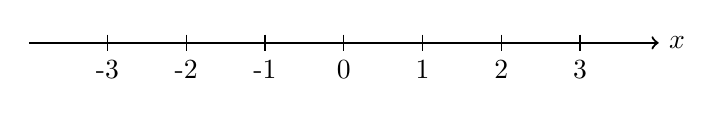
\begin{tikzpicture}
        \draw[thick,->] (-4.0,0) -- (4.0,0) node[right] {$x$}; % eje x
        \foreach \x in {-3,...,3}
        \draw (\x,3pt) -- (\x,-3pt)
        node[anchor=north] {\x};
        \end{tikzpicture}
    \end{center}
    \vskip 3cm 


    
\end{frame}


\begin{frame}
        
    Se puede usar un par de números $(x, y)$ para representar un punto en el plano\pause:
    {\footnotesize
    \begin{center}
        \begin{tikzpicture}[scale=1.1]
        \draw[thick,->] (-4.0,0) -- (4.0,0) node[right] {$x$}; % eje x
        \draw[thick,->] (0,-3) -- (0,3) node[above] {$y$}; % eje y
        \foreach \x in {-3,...,-1}
        \draw (\x,3pt) -- (\x,-3pt)
        node[anchor=north] {\x};
        \foreach \x in {1,...,3}
        \draw (\x,3pt) -- (\x,-3pt)
        node[anchor=north] {\x};
        \foreach \y in {-2,...,-1}
        \draw (3pt,\y) -- (-3pt,\y) 
        node[anchor=east] {\y}; 
        \foreach \y in {1,...,2}
        \draw (3pt,\y) -- (-3pt,\y)
        node[anchor=east] {\y}; 
        \draw[fill] (2,1) circle [radius=0.07];
        %\draw[thick,->] (0,0) -- (2,1);
        \node [right] at (2,1) {$(2,1)$};
        \draw [dashed] (0,1) -- (2,1);
        \draw [dashed] (2,0) -- (2,1);
        \draw[fill] (-1,2.5) circle [radius=0.07];
        %\draw[thick,->] (0,0) -- (-1,2.5);
        \node [left] at (-1,2.5) {$(-1,2.5)$};
        \draw [dashed] (0,2.5) -- (-1,2.5);
        \draw [dashed] (-1,0) -- (-1,2.5);
        \draw[fill] (-2.5,-2.5) circle [radius=0.07];
        %\draw[thick,->] (0,0) -- (-2.5,-2.5);
        \node [below] at (-2.5,-2.5) {$(-2.5,-2.5)$};
        \draw [dashed] (0,-2.5) -- (-2.5,-2.5);
        \draw [dashed] (-2.5,0) -- (-2.5,-2.5);
        \end{tikzpicture}
    \end{center}
}
\end{frame}



\begin{frame}
        Ahora observamos que un triple de números $(x, y, z)$ se puede usar para representar un punto en el espacio\pause:
        {\footnotesize
    \begin{center}
        \begin{tikzpicture}[scale=1]
        %draw the main coordinate system axes
        \draw[thick,->] (0,0,0) -- (5,0,0) node[right]{$y$};
        \draw[thick,->] (0,0,0) -- (0,4,0) node[above]{$z$};
        \draw[thick,->] (0,0,0) -- (0,0,5) node[anchor=north east]{$x$};

        %\draw[thick,->] (0,0,0) -- (3,2.5,3.5) node[anchor=west]{$v$};
        \draw [dashed] (0,2.5,0) -- (3,2.5,0);
        \draw [dashed] (0,2.5,0) --  (0,2.5,3.5);
        \draw [dashed] (0,2.5,3.5) -- (3,2.5,3.5) ;
        \draw [dashed] (3,0,0) -- (3,0.9,0);
        \draw [dashed] (3,1.5,0) -- (3,2.5,0);
        \draw [dashed] (0,0,3.5) -- (3,0,3.5);
        \draw [dashed] (0,0,3.5) -- (0,2.5,3.5);
        \draw [dashed] (3,0,3.5) -- (3,0,0);
        \draw [dashed] (3,2.5,3.5) -- (3,2.5,0);
        \draw [dashed] (3,2.5,3.5) -- (3,0,3.5);
        \foreach \y in {1,...,4}
        \draw (\y,0.1,0) -- (\y,-0.1,0)
        node[anchor=north] {\y};
        \foreach \y in {1,...,3}
        \draw (-0.1,\y,0) -- (0.1,\y,0)
        node[anchor=east] {\y\;};
        \foreach \y in {1,...,4}
        \draw (0.1,-0.1,\y) -- (-0.1,0.1,\y)
        node[anchor=south east] {\y\,};
        \draw[fill] (3,2.5,3.5) circle [radius=0.07] node[anchor=west]{\,$\mathbf{(3.5,3,2.5)}$};
        \end{tikzpicture}
    \end{center}            
    \pause
}
    En lugar de usar $(x,y,z)$, también suele usarse la notación $(x_1,x_2,x_3)$.
\end{frame}



\begin{frame}
    \begin{definicion}
        Sea $\R$ el cuerpo de los números reales,  entonces
        \begin{equation*}
        \R^n:= \{(x_1,x_2,\ldots,x_n): x_i \in \R, 1 \le i \le n \}.
        \end{equation*}
        Todo  $v$ en $\R^n$ será llamado {\em punto}\index{punto}. Alternativamente, también podemos decir que $v$  es un \textit{vector en el origen} o simplemente un \textit{vector}. 
    \end{definicion}
    
    \vskip .5 cm 
    \pause
    La mayoría de nuestros ejemplos tendrán lugar cuando $n = 2$ o $n = 3$. 
    \pause
    \vskip .5 cm 
    Para ello usaremos el {\em sistema  de coordenadas cartesianas}\index{sistema  de coordenadas cartesianas}\index{coordenadas cartesianas} para representar los elementos de  $\R^2$ y  $\R^3$.
\end{frame}



\begin{frame}
        \begin{ejemplo} \label{ej-3espacio-industria}
        El ministerio de economía quiere representar la inversión anual en 6 ramas de la industria:  1. acero, 2. automotriz, 3. productos agrícolas,  4. productos químicos, 5. indumentaria y 6. transporte. 
        
        \vskip .5 cm \pause
        Se puede representar esta situación por una $6$-upla donde cada coordenada representa la inversión anual de las industrias correspondientes. 
        \pause
        \vskip .5 cm 
        Por  ejemplo, si la 6-upla correspondiente al año 2019 es
        \begin{equation*}
        (1200, 700, 600, 300, 900, 250),
        \end{equation*}
        significa que la industria del acero invirtió 1200 en ese año, la automotriz 700, etc.
    \end{ejemplo} 
    
\end{frame}

\begin{frame}
    Recordemos que a los números complejos se los puede representar en el plano y  que la suma es \textit{coordenada a coordenada.}
    
    \vskip .3 cm \pause
    
    En  el ejemplo de la diapositiva anterior veamos que también es natural definir la suma coordenada a coordenada. 
    
    \vskip .3 cm \pause
    
    Por ejemplo, si las inversiones en los años  2018 y 2019 fueron  
    \begin{center}
        \begin{tabular}{lcl}
            2018 \quad&$\rightarrow$\quad &$(1000, 800, 550, 300, 700, 200)$ \\
            2019 \quad&$\rightarrow$\quad &$(1200, 700, 600, 300, 900, 250)$ 
        \end{tabular} 
    \end{center}
    Las inversiones totales, por rubro, en los dos años fueron: 
    \begin{align*}
    (&1000, 800, 550, 300, 700, 200) + (1200, 700, 600, 300, 900, 250) = \\
    &=(1000+1200, 800+700, 550+600, 300+300, 700+900, 200+250) \\
    &= (2200, 1500, 1350, 600, 1600, 450). 
    \end{align*} 
    
\end{frame}


\begin{frame}\frametitle{Suma en $\R^n$}
    
    \begin{block}{Definición 1.1.2}
        Si $(x_1,\ldots,x_n), (y_1,\ldots,y_n) \in \R^n$, definimos 
        \begin{equation*}
        (x_1,\ldots,x_n)+ (y_1,\ldots,y_n):=(x_1+y_1,\ldots,x_n+y_n),
        \end{equation*} 
        es decir sumamos ``coordenada a coordenada''.
    \end{block}
    
    
    \begin{exampleblock}{Ejemplo}
        En $\R^5$ tenemos que
        \begin{align*}
        (1,2,3,4,5)+(6,7,8,9,0)&=(1+6,2+7,3+8,4+9,5+0)\\
        &=(7,9,11,13,5)
        \end{align*}
        
    \end{exampleblock}
    
    
    
\end{frame}

\begin{frame}
    
    \begin{block}{Propiedades}
        La suma de vectores en $\R^n$ satisface que
        \begin{enumerate}
            \item Es asociativa:
            \begin{align*}
            u+(v+w)=(u+v)+w\quad\forall u,v,w\in\R^n
            \end{align*}
            \item Es conmutativa:
            \begin{align*}
            v + w = w + v\quad\forall v,w\in\R^n
            \end{align*}
            \item El vector ${0}: = (0,\dots,0)$, es el elemento \textit{neutro}: 
            \begin{align*}
            v +0 = 0 +v = v\quad\forall v\in\R^n
            \end{align*}
            
            \item El vector {$-v := (-x_1,\ldots, -x_n)$} es el \textit{opuesto} de $v = (x_1,\ldots,x_n)$:
            \begin{equation*}
            v + (-v) = (-v) + v = 0.
            \end{equation*}
        \end{enumerate}    
        
    \end{block}
    
    
\end{frame}

\begin{frame}
    Estas propiedades son consecuencias de las propiedades análogas de la suma de números reales. Pues la suma de vectores es coordenada a coordenada y las coordenadas son números reales.
    
    \vskip .3cm
    \pause 
    
    Por ejemplo, si {\footnotesize $u=(u_1, ..., u_n)$, $v=(v_1, ..., v_n)$, $w=(w_1, ..., w_n)$
    \pause
    \begin{align*}
    u+(v+w)&=(u_1, ..., u_n)+
    \biggl((v_1, ..., v_n)+(w_1, ..., w_n)\biggr)\\ 
    &=(u_1, ..., u_n)+(v_1+w_1, ..., v_n+w_n)\\
    &=\biggl(u_1+(v_1+w_1), ..., u_n+(v_n+w_n)\biggr)\\
    &=\biggl((u_1+v_1)+w_1, ..., (u_n+v_n)+w_n\biggr)\\
    &=(u_1+v_1, ..., u_n+v_n)+(w_1, ..., w_n)\\
    &=\biggl((u_1, ..., u_n)+
    (v_1, ..., v_n)\biggr)+(w_1, ..., w_n)\\
    &=(u+v)+w
    \end{align*}
}
\end{frame}



\begin{frame}\frametitle{Ley del paralelogramo}

        Sea $v =(2,3)$ y $w= (-1, 1)$. Entonces $v+w= (1, 4)$. En el dibujo de los puntos involucrados aparece un \textit{paralelogramo} 
        \pause
        \vskip .4cm
        
        {\footnotesize
        \begin{center}
            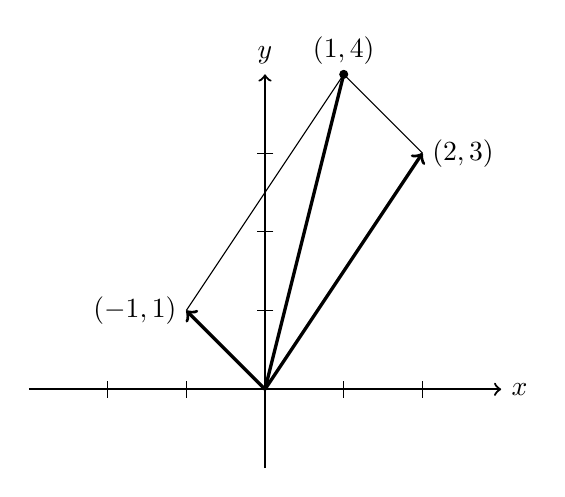
\begin{tikzpicture}[scale=1]
            \draw[thick,->] (-3.0,0) -- (3.0,0) node[right] {$x$}; % eje x
            \draw[thick,->] (0,-1) -- (0,4) node[above] {$y$}; % eje y
            \foreach \x in {-2,...,2}
            \draw (\x,3pt) -- (\x,-3pt);
            \foreach \y in {0,...,3}
            \draw (3pt,\y) -- (-3pt,\y) ;
            \draw[very thick, ->] (0,0) -- (-1,1);
            \node [left] at (-1,1) {$(-1,1)$};
            \draw[very thick,->] (0,0) -- (2,3);
            \node [right] at (2,3) {$(2,3)$};
            \draw[very thick,-] (0,0) -- (1,4);
            \node [above] at (1,4) {$(1,4)$};
            \draw[fill] (1,4) circle [radius=0.05];
            \draw[-] (-1,1) -- (1,4);
            \draw[-] (2,3) -- (1,4);
            \end{tikzpicture}
         \end{center} 
     }
\end{frame}



\begin{frame}
    En  general, la suma de dos vectores se puede representar geométricamente con la \textit{ley del paralelogramo}\pause:
    
    \vskip 1cm 
    
    
    \begin{center}
        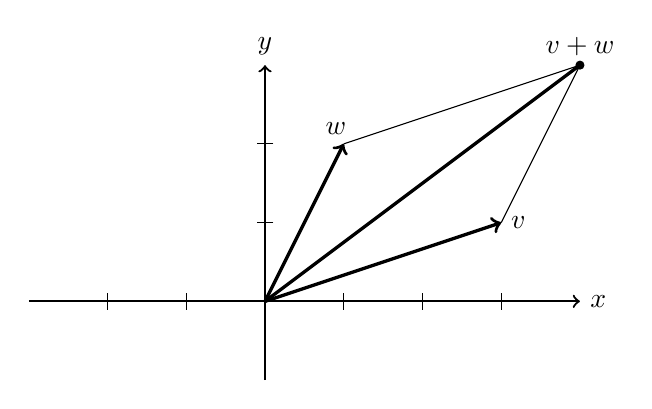
\begin{tikzpicture}[scale=1.0]
        \draw[thick,->] (-3.0,0) -- (4.0,0) node[right] {$x$}; % eje x
        \draw[thick,->] (0,-1) -- (0,3) node[above] {$y$}; % eje y
        \foreach \x in {-2,...,3}
        \draw (\x,3pt) -- (\x,-3pt);
        \foreach \y in {0,...,2}
        \draw (3pt,\y) -- (-3pt,\y) ;
        \draw[very thick, ->] (0,0) -- (3,1);
        \node [right] at (3,1) {$v$};
        \draw[very thick,->] (0,0) -- (1,2);
        \node [above] at (0.9,2) {$w$};
        \draw[very thick,-] (0,0) -- (4,3);
        \node [above] at (4,3) {$v+w$};
        \draw[fill] (4,3) circle [radius=0.05];
        \draw[-] (3,1) -- (4,3);
        \draw[-] (1,2) -- (4,3);
        \end{tikzpicture}
    \end{center}

\end{frame}



\begin{frame}\frametitle{El opuesto de un vector}
    El opuesto de un vector $v$  en el plano es $-v$ y geométricamente es el vector reflejado respecto al centro\pause:
    \begin{center}
        \begin{tikzpicture}[scale=1.0]
        \draw[thick,->] (-4.0,0) -- (4.0,0) node[right] {$x$}; % eje x
        \draw[thick,->] (0,-2) -- (0,2) node[above] {$y$}; % eje y
        \foreach \x in {-3,...,3}
        \draw (\x,3pt) -- (\x,-3pt);
        \foreach \y in {-1,...,1}
        \draw (3pt,\y) -- (-3pt,\y) ;
        \draw[very thick, ->] (0,0) -- (3,1);
        \node [right] at (3,1) {$v$};
        \draw[very thick, ->] (0,0) -- (-3,-1);
        \node [left] at (-3,-1) {$-v$};
        \draw[fill] (0,0) circle [radius=0.1];
        \end{tikzpicture}
    \end{center}
\end{frame}



\begin{frame}\frametitle{Resta de vectores}
    Dados dos  vectores $v$, $w$  en el plano, podemos representar la resta como la  suma de $v$ más el  opuesto de $w$, es decir 
    \begin{equation*}
        v-w :=  v + (-w).
    \end{equation*}
    \vskip .4 cm \pause
    Como $(v-w) + w = v$, la ley del paralelogramo también nos sirve para visualizar la resta.
    \pause
    
    \begin{center}
        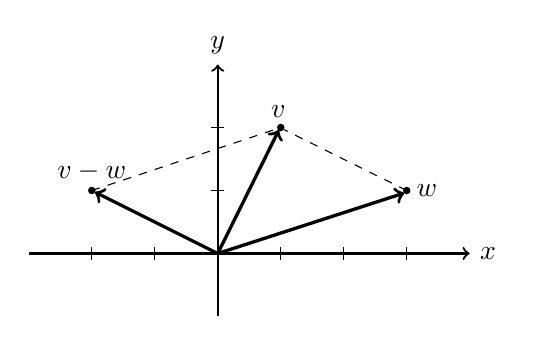
\begin{tikzpicture}[scale=0.8]
        \draw[thick,->] (-3.0,0) -- (4.0,0) node[right] {$x$}; % eje x
        \draw[thick,->] (0,-1) -- (0,3) node[above] {$y$}; % eje y
        \foreach \x in {-2,...,3}
        \draw (\x,3pt) -- (\x,-3pt);
        \foreach \y in {0,...,2}
        \draw (3pt,\y) -- (-3pt,\y) ;
        % vector w
        \draw[fill] (3,1) circle [radius=0.05];
        \node [right] at (3,1) {$w$};
        \draw[very thick, ->] (0,0) -- (2.96,0.96);
        % vector v
        \draw[fill] (1,2) circle [radius=0.05];
        \draw[very thick,->] (0,0) -- (0.97,1.96);
        \node [above] at (0.9,2) {\;$v$};
        % flecha punteada de w a v
        \draw[dashed] (3,1) -- (1.055,1.965);
        % vector v - w
        \draw[fill] (-2,1) circle [radius=0.05];
        \node [above] at (-2,1) {$v-w$};
        \draw[very thick,->] (0,0) -- (-2*0.975,1*0.975);    
        % punteada de v-w  a v
        \draw[dashed] (-2,1) -- (1,2);    
        \end{tikzpicture}
    \end{center}
\end{frame}



\begin{frame}\frametitle{Producto de un vector por un escalar}
    \begin{ejemplo}
        Sea $v= (1,2)$,  podemos representar los ``múltiplos''  de $v$ en forma natural: 
    \begin{center}
        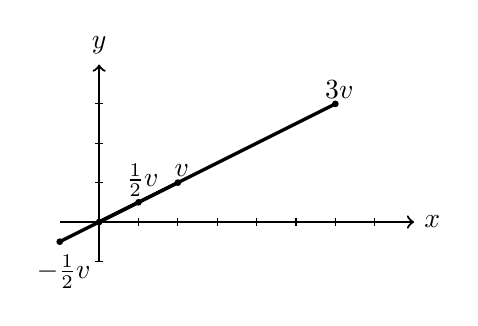
\begin{tikzpicture}[scale=0.5]
        \draw[thick,->] (-1,0) -- (8,0) node[right] {$x$}; % eje x
        \draw[thick,->] (0,-1) -- (0,4) node[above] {$y$}; % eje y
        \foreach \x in {0,...,7}
        \draw (\x,3pt) -- (\x,-3pt);
        \foreach \y in {-1,...,3}
        \draw (3pt,\y) -- (-3pt,\y) ;
        \def\vx{2}
        \def\vy{1}
        \draw[very thick, -] (0,0) -- (\vx,\vy);
        \node [above] at (\vx +0.1,\vy-0.1) {$v$};
        \draw[very thick, -] (0,0) -- (3*\vx,3*\vy);
        \node [above] at (3*\vx + 0.1,3* \vy-0.1) {$3v$};
        \draw[very thick, -] (0,0) -- (0.5*\vx ,0.5*\vy);
        \node [above] at (0.5*\vx + 0.1,0.5*\vy-0.1) {$\frac12v$};
        \draw[very thick, -] (0,0) -- (-0.5*\vx ,-0.5*\vy);
        \node [below] at (-0.5*\vx + 0.1,-0.5*\vy-0.1) {$-\frac12v$};
        \draw[fill] (0,0) circle [radius=0.07];
        \draw[fill] (0.5*\vx ,0.5*\vy) circle [radius=0.07];
        \draw[fill] (-0.5*\vx ,-0.5*\vy) circle [radius=0.07];
        \draw[fill] (3*\vx,3*\vy) circle [radius=0.07];
        \draw[fill] (\vx,\vy) circle [radius=0.07];
        \end{tikzpicture}
    \end{center}
        
        
    \end{ejemplo}
\end{frame}



\begin{frame}
    
    \begin{definicion}
        Sea $v = (x_1,\ldots,x_n) \in \R^n$ y $\lambda \in \R$, entonces
        \begin{equation*}
        \lambda.v = (\lambda x_1,\ldots,\lambda x_n).
        \end{equation*}  
        También denotamos a esta multiplicación por $\lambda v$.
    \end{definicion}
    \vskip .4 cm \pause
    \begin{ejemplo}
        Si $v= (2, -1.5)$  y $\lambda = 7$, entonces $\lambda v = (14, -10.5)$.
    \end{ejemplo}
    \vskip 2 cm
\end{frame}




\begin{frame}
    
    \begin{block}{Propiedades}
        La multiplicación por escalares satisface que
        \begin{enumerate}
            \item Es asociativa
            \begin{align*}
            (\lambda\mu)v&= \lambda(\mu v)\quad\forall v\in\R^n,\,\lambda,\mu\in\R.
            \end{align*}
            \pause
            \item Es distributiva
            \begin{align*}
            \lambda (v + w) &= \lambda v + \lambda w\quad\forall v,w\in\R^n,\,\lambda\in\R\\
            (\lambda+\mu)v&= \lambda v + \mu v\quad\forall v\in\R^n,\,\lambda,\mu\in\R
            \end{align*}
        \end{enumerate}
    \end{block}
    
    \
    \pause
    Al igual que las propiedades de la suma, estas también se deducen de las propiedades de los números.
    
    \
    \pause
    Similarmente, multiplicando por $(-1)$ obtenemos el opuesto:
    \begin{equation*}
    (-1)v = -v\quad\forall v\in\R^n.
    \end{equation*}
\end{frame}


\begin{frame}

    \begin{block}{Definición}
        Sean  $v_1, \ldots, v_k$ vectores en $\R^n$. Una  \textit{combinación lineal de $v_1, \ldots, v_k$} es un vector de la forma
        \begin{equation*}
        \lambda_1v_1 + \cdots + \lambda_kv_k,
        \end{equation*}
        donde $\lambda_1, \ldots, \lambda_k$ son números reales.
    \end{block}
    
    \begin{exampleblock}{Ejemplo}
        En $\R^3$, sean los vectores  $v_1 = (1,2,3)$, $v_2=(-1,3,0)$, $v3 = (-1,-0,1)$ y $v_4 = (-2,-1,-3)$ entonces
        \begin{align*}
            v &= 2v_1 - 3v_2 + 4v_3 - 5v_4\\
            &= 2(1,2,3) - 3(-1,3,0) + 4(-1,0,1) - 5(-2,-1,-3)\\
            &= (2,4,6) + (3,-9,0) + (-4,0,4) + (10,5,15)\\
            &= (11,0,25),
        \end{align*}
        es una combinación lineal de $v_1, v_2, v_3, v_4$.
    \end{exampleblock}
    
\end{frame}

\begin{frame}
    
    \begin{exampleblock}{Definición}
        
        Dado $i\in\{1, ..., n\}$, se denota ${e_i}\in\R^n$ al vector cuyas coordenadas son todas $0$ excepto la coordenada $i$ que es un $1$.
        \begin{align*}
        e_i=(0, ..., 1, ..., 0)
        \end{align*}
        El conjunto $\{e_1, ..., e_n\}$ se llama\textit{ {base canónica}} de $\R^n$.
    \end{exampleblock}
    
    \begin{exampleblock}{Ejemplo}
        En $\R^3$ los vectores son $
        e_1=(1,0,0)$, $
        e_2=(0,1,0)$, 
        $e_3=(0,0,1)
        $
    \end{exampleblock}
    
    \
    
    Estos vectores jugarán un rol central en la materia.
    
    \
    
    Principalmente, por la siguiente propiedad.
    
\end{frame}


\begin{frame}

    \begin{block}{Propiedad}
        Todo vector de $\R^n$ se escribe como combinación lineal de la base canónica. Explicitamente, si $(x_1, ..., x_n)\in\R^n$ entonces
        \begin{align*}
        (x_1, ..., x_n)=x_1e_1+x_2e_2+\cdots+x_ne_n
        \end{align*}
    \end{block}
    
    \
    
    La demostración es trivial pero por ahora no la haremos. 
    
    
    \begin{exampleblock}{Ejemplo}
        
        \begin{align*}
        (1,2,3)&=(1,0,0)+(0,2,0)+(0,0,3)\\
        &=1(1,0,0)+2(0,1,0)+3(0,0,1)\\
        &=1e_1+2e_2+3e_3
        \end{align*}
        
    \end{exampleblock}
    
    
\end{frame}



\end{document}

